\section{Results} \label{sec:6results}
This section presents the analysis results of the previous three cases and compares them with
models from the literature.
Our experiment was conducted on a server running Ubuntu 22.04 with an AMD 7950X3D CPU and
192GB RAM.
We used \Tamarin{} as the unmodified verification backend, and EntropyVerif operates purely as
a source-to-source front-end that emits standard \Tamarin{} input.
The source models, the generated models and our own runs are in the repository~\cite{toolrepo},
which also ships the container images that pin the toolchains we used.
We will provide a detailed description of the process for the novel attack discovered from the
BC analysis results.

\subsection{WPA2-PSK}

\cite{cremers2020wpa2}'s formal analysis of the WPA2 protocol revealed its vulnerability to Kracks~(Key Reinstallation Attacks)\cite{vanhoef2017krack}.
While the original study primarily focused on the impact of nonce reuse on protocols, we made slight modifications to their formal model to apply our methodology proposed in this paper.
These modifications enable the attacker to compromise low-entropy keys, allowing us to investigate the security vulnerabilities arising from the misuse of common passwords.
This approach provides an understanding of the potential risks associated with low-entropy key
exploitation.

\begin{table}[ht]
    \centering
    \caption{ Analysis Results of WPA2-PSK } \label{tab:4-way-handshake-result}
    \renewcommand{\arraystretch}{1.2} \setlength{\tabcolsep}{8pt}
    \begin{threeparttable}[b]
        \begin{tabular}{lccc}
        \hline
        Model & Executability & PMKID Attack & Kracks \\
        \hline
        \cite{cremers2020wpa2}'s Model & \textcolor{xhs_green}{\ding{52}} & \textcolor{xhs_green}{\ding{52}} & \textcolor{xhs_red}{\ding{56}} \\
        Our Model & \textcolor{xhs_green}{\ding{52}} & \textcolor{xhs_red}{\ding{56}} & \textcolor{xhs_red}{\ding{56}} \\
        \hline
        \end{tabular}
        \begin{tablenotes}
            \item[] \textcolor{xhs_green}{\ding{52}}: the property is satisfied. \hspace{1em} 
                    \textcolor{xhs_red}{\ding{56}}: the property is falsified.
        \end{tablenotes}
    \end{threeparttable}
\end{table}

As shown in \autoref{tab:4-way-handshake-result}, 
our model can discover not only Kracks same as the original one but also the PMKID attack, which was not apparent in the original analysis results.

\begin{table*}[t]
    \centering
    \caption{Analysis Results of BLE Pairing} \label{tab:ble-pairing-result}
    \renewcommand{\arraystretch}{1.2} \setlength{\tabcolsep}{8pt}
    \begin{threeparttable}[b]
        \begin{tabular}{lccccccc}
            \hline  
            Model & Executability & Auth. of Initiator's LTK & Auth. of Responder's LTK & MitM Protection & Secrecy of LTK \\
            \hline  
            Model in \cite{shi2023blesc} + Session & \textcolor{xhs_green}{\ding{52}} & \textcolor{xhs_red}{A1} & \textcolor{xhs_red}{A1} & \textcolor{xhs_red}{A1} & \textcolor{xhs_green}{\ding{52}}  \\
            Our Model + Session & \textcolor{xhs_green}{\ding{52}} & \textcolor{xhs_red}{A2} & \textcolor{xhs_red}{A2} & \textcolor{xhs_red}{A1} & \textcolor{xhs_red}{A2}  \\
            \hline  
        \end{tabular}
        \begin{tablenotes}
            \item[] \textcolor{xhs_red}{A1}: Method Confusion Attack\cite{von2021method} \hspace{1em}
                    \textcolor{xhs_red}{A2}: Key Negotiation of Bluetooth~(KNOB) Attack\cite{antonioli2019knob} \hspace{1em}
                    \textcolor{xhs_green}{\ding{52}}: the property is satisfied. 
        \end{tablenotes}
    \end{threeparttable}
\end{table*}

\subsection{Pairing of BLE}
There are many formal analysis works\cite{ wu2022formal,shi2023blesc, claverie2023tamarin,jangid2023bluepe} on BLE-SC pairing protocols using \Tamarin{}.
Among these, the symbolic model proposed in \cite{shi2023blesc} stands out as the most comprehensive one.
This work introduced several security properties, including four authentication properties, man-in-the-middle~(MitM) protection, LTK confusion protection, and the secrecy of LTK.
However, the approach taken in this work to model brute-force attacks is tricky and imprecise due to the oversimplification of the key transmission process within the pairing protocol.

We corrected their work by modeling the establishment of encrypted sessions and the transmission of keys and then applied our methodology to the complemented model. 
All the analysis results of the two models are shown in \autoref{tab:ble-pairing-result}.
Our model can discover both the  KNOB attack and Method Confusion Attack\cite{von2021method} which is ignored by the complemented version of \cite{shi2023blesc}'s model.

\subsection{Session Establishment of BC}
We performed a study of the session establishment protocol of BC by analyzing several scenarios under the QA and SA models and the results of our analysis are summarized in \autoref{tab:bc-session-result}.
% 我们发现，BC会话的安全性主要取决于边缘设备最低支持的密钥长度，只要边缘设备支持的最低密钥长度在攻击者妥协的长度范围之内，边缘设备的会话密钥就一定会被妥协。当边缘设备兼容legacy设备时，情况会更加糟糕：即使双方协商出了最长的会话密钥，攻击者也可以通过多次降级边缘设备的密钥，来恢复出完整的会话密钥，即使该密钥的长度远超攻击者的计算能力。

We have found that the security of BC sessions largely depends on the minimum key length supported by peripheral devices. 
As long as this minimum key length falls within the range that an attacker can compromise, the session key of the peripheral device will inevitably be compromised. 
The situation worsens when the peripheral device is compatible with legacy devices: 
an attacker can repeatedly downgrade the peripheral device's key, ultimately recovering the longest session key, even if the key length far exceeds the attacker’s computational capacity.
This attack against BC devices isn't covered by the existing literature, and we term it the Unilateral Multi-Downgrade(UMD) attack.

\begin{table*}[t]
    \centering
    \caption{Analysis Results of BC Session Establishment Protocol} \label{tab:bc-session-result}
    \renewcommand{\arraystretch}{1.2} \setlength{\tabcolsep}{8pt}
    \begin{threeparttable}[b]
    \begin{tabularx}{\textwidth}{c>{\centering\arraybackslash}X>{\centering\arraybackslash}X>{\centering\arraybackslash}X>{\centering\arraybackslash}X>{\centering\arraybackslash}X>{\centering\arraybackslash}X}
    \hline
    Session Scenario & Adversary Model & SecCenSK & SecPerSK & MitMResistance & Time (s) \\ 
    \hline
    \makebox[2.25em][s]{L\hfill g\hfill O\hfill n}\hspace{0.1em}-\hspace{0.1em}\makebox[2.9em][s]{L\hfill e\hfill g\hfill a\hfill c\hfill y}\hspace{0.5em}$\times$\hspace{0.5em}\makebox[2.25em][s]{L\hfill g\hfill O\hfill n}\hspace{0.1em}-\hspace{0.1em}\makebox[2.9em][s]{L\hfill e\hfill g\hfill a\hfill c\hfill y} & QA & \textcolor{xhs_red}{A1} & \textcolor{xhs_red}{A1} & \textcolor{xhs_red}{A1} & 18.43 \\
    \makebox[2.25em][s]{L\hfill g\hfill O\hfill n}\hspace{0.1em}-\hspace{0.1em}\makebox[2.9em][s]{L\hfill e\hfill g\hfill a\hfill c\hfill y}\hspace{0.5em}$\times$\hspace{0.5em}\makebox[2.25em][s]{L\hfill g\hfill O\hfill n}\hspace{0.1em}-\hspace{0.1em}\makebox[2.9em][s]{E\hfill n\hfill h\hfill a\hfill n\hfill c} & QA & \textcolor{xhs_green}{\ding{52}}  & \textcolor{xhs_green}{\ding{52}}  & \textcolor{xhs_green}{\ding{52}}  & 99172.49 \\
    \makebox[2.25em][s]{L\hfill g\hfill O\hfill n}\hspace{0.1em}-\hspace{0.1em}\makebox[2.9em][s]{E\hfill n\hfill h\hfill a\hfill n\hfill c}\hspace{0.5em}$\times$\hspace{0.5em}\makebox[2.25em][s]{L\hfill g\hfill O\hfill n}\hspace{0.1em}-\hspace{0.1em}\makebox[2.9em][s]{L\hfill e\hfill g\hfill a\hfill c\hfill y} & QA & \textcolor{xhs_red}{A2} & \textcolor{xhs_red}{A2} & \textcolor{xhs_red}{A2} & 32.95 \\
    \makebox[2.25em][s]{L\hfill g\hfill O\hfill n}\hspace{0.1em}-\hspace{0.1em}\makebox[2.9em][s]{S\hfill e\hfill c\hfill u\hfill r\hfill e}\hspace{0.5em}$\times$\hspace{0.5em}\makebox[2.25em][s]{L\hfill g\hfill O\hfill n}\hspace{0.1em}-\hspace{0.1em}\makebox[2.9em][s]{L\hfill e\hfill g\hfill a\hfill c\hfill y} & QA & \textcolor{xhs_red}{A2} & \textcolor{xhs_red}{A2} & \textcolor{xhs_red}{A2} & 81.19 \\
    \makebox[2.25em][s]{S\hfill c\hfill L\hfill g}\hspace{0.1em}-\hspace{0.1em}\makebox[2.9em][s]{S\hfill e\hfill c\hfill u\hfill r\hfill e}\hspace{0.5em}$\times$\hspace{0.5em}\makebox[2.25em][s]{S\hfill c\hfill L\hfill g}\hspace{0.1em}-\hspace{0.1em}\makebox[2.9em][s]{L\hfill e\hfill g\hfill a\hfill c\hfill y} & QA & \textcolor{xhs_red}{A2} & \textcolor{xhs_red}{A2} & \textcolor{xhs_red}{A2} & 150.13 \\
    \makebox[2.25em][s]{S\hfill c\hfill L\hfill g}\hspace{0.1em}-\hspace{0.1em}\makebox[2.9em][s]{S\hfill e\hfill c\hfill u\hfill r\hfill e}\hspace{0.5em}$\times$\hspace{0.5em}\makebox[2.25em][s]{S\hfill c\hfill L\hfill g}\hspace{0.1em}-\hspace{0.1em}\makebox[2.9em][s]{E\hfill n\hfill h\hfill a\hfill n\hfill c} & QA & \textcolor{xhs_green}{\ding{52}}  & \textcolor{xhs_green}{\ding{52}}  & \textcolor{xhs_green}{\ding{52}}  & 83574.33 \\
    \makebox[2.25em][s]{S\hfill c\hfill O\hfill n}\hspace{0.1em}-\hspace{0.1em}\makebox[2.9em][s]{S\hfill e\hfill c\hfill u\hfill r\hfill e}\hspace{0.5em}$\times$\hspace{0.5em}\makebox[2.25em][s]{S\hfill c\hfill O\hfill n}\hspace{0.1em}-\hspace{0.1em}\makebox[2.9em][s]{L\hfill e\hfill g\hfill a\hfill c\hfill y} & QA & \textcolor{xhs_green}{\ding{52}}  & \textcolor{xhs_red}{A1} & \textcolor{xhs_green}{\ding{52}}  & 3993.54 \\
    \makebox[2.25em][s]{S\hfill c\hfill O\hfill n}\hspace{0.1em}-\hspace{0.1em}\makebox[2.9em][s]{S\hfill e\hfill c\hfill u\hfill r\hfill e}\hspace{0.5em}$\times$\hspace{0.5em}\makebox[2.25em][s]{S\hfill c\hfill O\hfill n}\hspace{0.1em}-\hspace{0.1em}\makebox[2.9em][s]{E\hfill n\hfill h\hfill a\hfill n\hfill c} & QA & \textcolor{xhs_green}{\ding{52}}  & \textcolor{xhs_green}{\ding{52}}  & \textcolor{xhs_green}{\ding{52}}  & 13319.46 \\
    \hline
    \makebox[2.25em][s]{L\hfill g\hfill O\hfill n}\hspace{0.1em}-\hspace{0.1em}\makebox[2.9em][s]{S\hfill e\hfill c\hfill u\hfill r\hfill e}\hspace{0.5em}$\times$\hspace{0.5em}\makebox[2.25em][s]{L\hfill g\hfill O\hfill n}\hspace{0.1em}-\hspace{0.1em}\makebox[2.9em][s]{L\hfill e\hfill g\hfill a\hfill c\hfill y} & SA & \textcolor{xhs_red}{A2} & \textcolor{xhs_red}{A2} & \textcolor{xhs_red}{A2} & 82.68 \\
    \makebox[2.25em][s]{S\hfill c\hfill L\hfill g}\hspace{0.1em}-\hspace{0.1em}\makebox[2.9em][s]{S\hfill e\hfill c\hfill u\hfill r\hfill e}\hspace{0.5em}$\times$\hspace{0.5em}\makebox[2.25em][s]{S\hfill c\hfill L\hfill g}\hspace{0.1em}-\hspace{0.1em}\makebox[2.9em][s]{L\hfill e\hfill g\hfill a\hfill c\hfill y} & SA & \textcolor{xhs_red}{A2} & \textcolor{xhs_red}{A2} & \textcolor{xhs_red}{A2} & 67.50 \\
    \makebox[2.25em][s]{S\hfill c\hfill O\hfill n}\hspace{0.1em}-\hspace{0.1em}\makebox[2.9em][s]{S\hfill e\hfill c\hfill u\hfill r\hfill e}\hspace{0.5em}$\times$\hspace{0.5em}\makebox[2.25em][s]{S\hfill c\hfill O\hfill n}\hspace{0.1em}-\hspace{0.1em}\makebox[2.9em][s]{L\hfill e\hfill g\hfill a\hfill c\hfill y} & SA & \textcolor{xhs_green}{\ding{52}}  & \textcolor{xhs_red}{A1} & \textcolor{xhs_green}{\ding{52}}  & 50789.74 \\
    \hline
    \end{tabularx}
    \begin{tablenotes}
        \item[] 
        \begin{itemize}[leftmargin=*]
            \item   \hspace{0.25em} A1: Key Negotiation of Bluetooth~(KNOB) Attack\cite{antonioli2019knob} 
                    \hspace{1em} A2: novel Unilateral Multi-Downgrade Attack 
                    \hspace{1em} \textcolor{xhs_green}{\ding{52}}: the property is satisfied. 
            \item   \hspace{0.25em} ScLg: support both secure and legacy connections.
                    \hspace{1em} ScOn: only support secure connections.
                    \hspace{1em} LgOn: only support legacy connections.
            \item   \hspace{0.25em} Legacy, Enhanc, Secure: key length ranges, see \autoref{sec:bc-devices} for details.
        \end{itemize}
        % A1: Key Negotiation of Bluetooth~(KNOB) Attack\cite{antonioli2019knob} 
        % \hspace{1em} A2: novel Unilateral Multi-Downgrade Attack 
        % \hspace{1em} \textcolor{xhs_green}{\ding{52}}: the property is satisfied.  \\
        % ScLg: support both secure and legacy connections.
        % \hspace{1em} ScOn: only support secure connections.
        % \hspace{1em} LgOn: only support legacy connections. \\
        % Legacy, Enhanc, Secure: key length ranges, see \autoref{sec:bc-devices} for details.
    \end{tablenotes}
    \end{threeparttable}
\end{table*}

\subsection{The Unilateral Multi-Downgrade Attack} \label{sec:umd-attack}
% 我们的模型发现了这个新攻击，其中，攻击者多次降级一侧设备的密钥长度，以分段地恢复出完整的会话密钥。在一个理想的BC会话建立协议中，一个仅接受16字节密钥的中心设备和接受1-16字节的边缘设备协商的会话密钥长度为16字节，攻击者很难通过暴力手段破解。但是，攻击者首先将双方降级到Legacy会话，然后将边缘设备的密钥降级到8字节，暴力破解出8字节的会话密钥。然后，重新与边缘设备建立会话，将会话密钥升级到16字节，这样，攻击者就可以通过暴力破解的方式破解出剩余的8字节会话密钥。整个过程如图\autoref{fig:bc-umd}所示。
We discover this novel attack where an attacker incrementally downgrades the key length of a device on one side to recover the complete session key.
% In an ideal BC session establishment procedure, a central device that only accepts a 16-byte key and a peripheral device that accommodates key lengths from 1 to 16 bytes negotiate a session key length of 16 bytes, rendering brute-force attacks impractical.
Given a central device that only accepts 16-byte keys and a peripheral device that supports key lengths from 1 to 16 bytes, their negotiated session key can only be 16 bytes long, making brute-force attacks infeasible.  
Nevertheless, the attacker initiates the attack by downgrading both devices to a Legacy session.
The attacker then induces the peripheral device to use a 4-byte session key, allowing the attacker to brute-force the first 4 bytes of the session key. 
Subsequently, the attacker repeats this process three times, ultimately recovering the complete session key. 
The complete process is depicted in \autoref{fig:bc-umd}.
\begin{figure}[t]
    \centering
    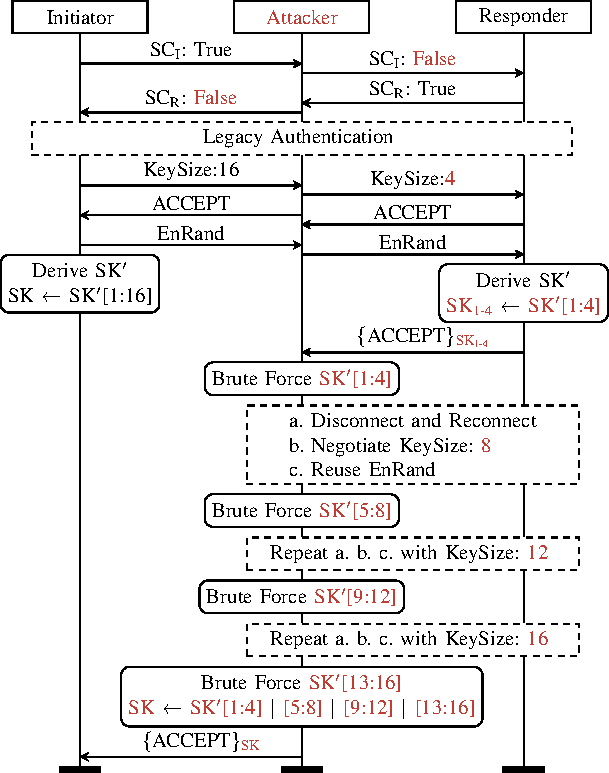
\includegraphics[width=0.945285\columnwidth]{img/umd-attack} 
    \caption{Attack flow of UMD attack on BC session establishment}
    \label{fig:bc-umd}
\end{figure}

% the UMD attack 有很多变体，攻击者可以根据自己的计算能力和受害设备最低支持的密钥长度，自由选择逐步降级的次数。假设攻击者选择的降级次数为$n$，每次降级的大小间隔一致，那么攻击者的计算次数为$2^{\frac{128}{n}}n$，当n为16时，攻击者暴力破解16字节的会话密钥的难度从$2^{128}$次降到$2^{12}$次。
The UMD attack encompasses several variations, allowing the attacker to freely choose the number of downgrade steps based on their computational resources and the minimum key length supported by the victim device.
If the attacker chooses $n$ downgrade steps, with each step having a consistent interval, the number of computations required by the attacker is $n \times 2^{\frac{128}{n}}$.
When $n$ is 16, the complexity of brute-forcing a 16-byte session key is significantly reduced from $2^{128}$ to $2^{12}$.

The discovery of the UMD attack implies that even if the central device only accepts 16-byte session keys, an attacker can still compromise the session key.
This attack highlights the inherent risks associated with compatibility with legacy devices, as it enables attackers to compromise session keys without eventually downgrading them.

\subsection{Performance Evaluation} \label{sec:performance}

This subsection reports what our translation costs on protocols that contain a low-entropy value
but no reachable brute-force attack, and where the additional proof effort goes.

\noindent\textbf{Protocols with no reachable attack.}
To see what the translation costs when there is nothing to find, we applied EntropyVerif to three
models of the Alipay payment protocols developed by Xiao et al.~\cite{xiao2026payment}: payment
from the mobile application, payment from the mobile web page, and payment by scanning an order
code.
All three carry a user payment password, which is low entropy, but none of them exposes a function
output from which the password could be recomputed.
The change to each model is one label marking the password as low entropy.
Every lemma reaches the same verdict as in the unannotated model and the finished proofs have the
same number of steps, so the analysis outcome does not change. The annotation adds about twelve
seconds to the two simpler models and about four minutes to the order-code model.
Appendix~\ref{app:alipay-time} gives the times.

\noindent\textbf{Where the proof effort goes.}
\Tamarin{} solves constraints in an interdependent way, so its running time cannot be divided
among individual goals. We therefore count the proof steps of each verified BC lemma and assign
each step to the goal it solves. The facts our translation adds take 86.4\% of the steps, and the
goals of the protocol model itself take 54 out of 1{,}779{,}376. Those steps are not new
cryptographic reasoning: a derivation goal asks which terms an observed message was computed from,
and 72\% of them are closed by a rule of the protocol model, so the cost grows with the number of
rules that could have produced a message rather than with the number of low-entropy keys.
Recovering a key is itself almost free, at 0.28\% of the steps. Appendix~\ref{app:breakdown} gives the
method and the per-lemma split.

\noindent\textbf{Human guidance.}
Two kinds of input are supplied by hand, and neither is a lemma.
The first is the low-entropy labeling, which asks for protocol knowledge: for BC, that the session
key is assembled from parts whose lengths the two sides agree on separately.
The second is a heuristic tactic that adjusts goal and branch priorities so that infeasible
branches are closed earlier. It deprioritizes the brute-force goals involving \TFact{MDerive} and
\TFact{EntropyLow}, letting \Tamarin{} analyze them after the others. A tactic restricts no trace
the model admits, so a proof that closes means the same with it as without it.
This strategy is general, although applying it takes minor adjustments for each model: six lines
in each BLE tactic and fourteen in BC. The BC models use tactics alone and carry one, identical in
the SA and QA templates, so all eleven configurations use it, not only the slow ones.

